%% The first command in your LaTeX source must be the \documentclass command.
%%
%% Options:
%% twocolumn : Two column layout.
%% hf: enable header and footer.
\documentclass[
% twocolumn,
% hf,
]{aiitart}
\usepackage{doi}
\def\doitext{DOI:}
\usepackage{indentfirst}

    \usepackage{unicode-math}
    \defaultfontfeatures{Ligatures=TeX}
    \setmathfont{Latin Modern Math}
    \setmainfont{Times New Roman}
    \setmonofont{Fira Mono}[Scale=MatchLowercase]



%%
%% One can fix some overfulls
\sloppy

%%
%% Minted listings support
%% Need pygment <http://pygments.org/> <http://pypi.python.org/pypi/Pygments>
\usepackage{minted}

%% auto break lines
% \lstset{breaklines=true}
%%
%% end of the preamble, start of the body of the document source.
\newcommand{\email}[1]{\texttt{#1}}
\graphicspath{{pics/}}
\providecommand{\LuaLaTeX}{Lua\LaTeX}

\begin{document}

%%
%% Rights management information.
%% CC-BY is default license.
%\copyrightyear{2022}
% \copyrightclause{Copyright for this paper by its authors.  Use permitted under Creative Commons License Attribution 4.0  International (CC BY 4.0).}
%%
%% This command is for the conference information
\conference{AIIT'2022 14 октября 2022 года, Зренянин, Сербия}

%%
%% The "title" command
\title{Распределенная инфраструктура на основе графа знаний для обработки документов, используемых для организации образовательного процесса}

% Менять можно все, и заголовок.... мы тут сами по себе
%%
%% The "author" command and its associated commands are used to define
%% the authors and their affiliations.
\author[1,2]{Евгений Черкашин} \author[2]{Виктория Попова}

% \cormark[1]
% \fnmark[1]
\address[1]{Институт динамики систем и теории управления им. В.М. Матросова СО ран, Иркутск, Россия} \address[2]{Институт математики и информационных технологий, Иркутский государственный университет, Иркутск, Россия\\[0.7em] \email{eugeneai@icc.ru};\quad\email{victorypopova1@gmail.com}}

%% Footnotes
% \cortext[1]{Corresponding author.}
%\fntext[1]{These authors contributed equally.}

%%
%% The abstract is a short summary of the work to be presented in the
%% article.
\begin{abstract}
В статье рассматривается применение ранее разработанных инфраструктурных компонентов, основанных на представлении данных в графе знаний и обработке данных, основанной на знаниях, для обработки документов университетского курса, их создания и обеспечения их данными будущей платформы для организации образовательного процесса. Основной целью является интеграция статических данных сайта университета, представленных в виде документации образовательной программы, с университетской инфраструктурой, например, библиотекой, расписанием, различными существующими системами планирования процессов, уже сделанными магистрантами и профессорско-преподавательским составом института.
\end{abstract}

%%
%% Keywords. The author(s) should pick words that accurately describe
%% the work being presented. Separate the keywords with commas.
\begin{keywords}
граф знаний \sep логический вывод \sep автоматизация образовательного процесса \sep распределенная обработка данных \sep автоматизация создания документов
\end{keywords}

%%
%% This command processes the author and affiliation and title
%% information and builds the first part of the formatted document.
\maketitle

%     July 2020
% DOI:10.47350/ICCS-DE.2020.24
%    Proceedings of The International Workshop on Information, Computation, and Control Systems for Distributed Environments
\section{Введение}

Университет представляет собой сложную социотехническую систему (СТС), \cite{zh2020} состоящую из различных компонентов, функционирование которой обеспечивается персоналом с использованием программного обеспечения. Иркутский государственный университет (ИГУ) имеет достаточный (требуемый) уровень автоматизации в областях бухгалтерского учета, планирования образовательного процесса, управления образовательным процессом, оценки успехов обучения студентов, доступа к библиотечным данным. Автоматизация имеет островной характер как в смысле функций предметной области, так и структурном смысле. Институты ИГУ разрабатывают свое собственное программное обеспечение для решения своих текущих технических проблем и не делятся результатами между институтами. Кажется, что такой традиции не существует. Решения, имеющие комплексный характер, реализуются специальным отделом Института математики и информационных технологий (ИМИТ) по договоренности. Например, во время пандемии COVID-19 ИМИТ поддерживал функционирование сервера Big Blue Button для всех подразделений ИГУ, спроектировал и внедрил модули Moodle для удаленного управления регистрацией абитуриентов.

% Неправильные термимны
% syllabus - sillabi (pl.) = Рабочая прграмма дисциплины.
% Syllabus: A list of topics or books that are planned to be studied in a particular subject.
% curriculum - curricula (pl.) = учебный план.
% Curriculum: The subjects that are included in a course of study in a college or university. (noun)
% faculty - профессорско-преподавательский состав (ППС)
% Faculty: A group of departments in a college or university that focuses on an area of study or several related subjects. (noun)
% appraisal fund - ФОС
Для того чтобы обеспечить выполнение постоянно растущих требований, предъявляемым к функционированию университета, необходимо устранить очевидные недостатки автоматизации учебного процесса. Одной из сложных проблем является подготовка документации курса, например, рабочих программ дисциплин (РПД), точно соответствующих учебному плану (УП) конкретной студенческой группы. При сокращении или изменении количества зачетных единиц (часов) в УП, затраченных на лекции и лабораторные работы, преподаватель должен изменить их количество в РПД, добавив / удалив темы или сократив / расширив их содержание. Формат представления РПД меняется примерно каждые два года, и даже статическая часть текста, как правило, подвергается некоторой реконструкции. Еще одна задача заключается в проверке возможностей университетской библиотеки по предоставлению печатных изданий (книгообеспеченность), верификация существования, доступности материала и обновление ссылок на электронные издания. Другая проблема связана с управлением образовательным процессом. Отсутствует общая система планирования и просмотра расписания занятий, мониторинга успеваемости учащихся, а именно факта посещения занятия и ведение перечня полученных оценок.

% Some departments have their localized solutions, which cannot be efficiently adapted.% Другой проблемой, которую требуется решить непосредственно по части организации учебного процесса, является отсутствие единой информационной системы, которая бы позволила просматривать расписание занятий, а также контролировать успеваемость студентов за счёт выставления оценок и отметок о посещаемости занятий. Важно отметить, что некоторыми учебными подразделениями такие проблемы уже решены. Но разработанные информационные системы адаптированы под характеристики конкретного учебного подразделения, что не позволяет использовать ту же систему в другом подразделении. Поэтому требуются такие программные продукты, которые могли бы использовать все институты и факультеты ИГУ для решения проблем организации учебного процесса.

Вышеупомянутые проблемы решаются преподавателями вручную с использованием программного обеспечения автоматизации делопроизводства (Microsoft и LibreOffice).  Руководство института разрабатывает рекомендации и шаблоны документов для поддержки деятельности преподавателей своевременно разрабатывать и обновлять РПД: создавать документы требуемого качества (во всех аспектах). Разработанные вручную расписания занятий публикуются на сайте ИГУ сразу после их формирования. Человеческий фактор проявляется в ухудшении качества выполнения требований. Частично это связано с нынешней недооценкой роли преподавателя и экономическими причинами: преподаватели часто работают в других учреждениях (институтах, вузах, фирмах), и работа с документами не является их основным приоритетом в организации рабочего времени.

% In such circumstances, its reconstruction becomes inoperative.   %  Что касается задач представления расписания и контроля успеваемости студентов, такие задачи также часто решаются вручную при помощи продуктов Microsoft и LibreOffice, из-за чего  редактирование расписания занятий является неоперативным процессом, поскольку изменения будут отображаться студентам и преподавателям только после публикации документа на веб-сайте или на стенде института. При достаточном количестве человеческих ресурсов такого вида работы могут быть выполнены оперативно с низкой вероятностью возникновения ошибок.
Кажется, что проблемы можно решить, используя искусственный интеллект для атоматизации создания документов. Согласно законодательству РФ ИГУ включает разделы для предоставления студентам и преподавателям документов об учебном процессе, включая УП и РПД за последние несколько лет по всем учебным программам и группам студентов. Документы представлены в формате PDF, они представляют собой источниками содержательных данных.  Другая полезная информация представлена документами на сайтах Правительства РФ, в том числе справочниками по специальностям, требованиям к специальностям и т.п.

Другие вышеупомянутые проблемы планирования занятий и мониторинга успеваемости учащихся требуют автоматизации во многих аспектах, включая использование механизмов комбинаторной оптимизации для решения задачи составления расписаний (подкласс задач удовлетворения ограничений), представление данных для оценок учащихся (формальных и инструктивных), их содержательное описание, соответствие образовательным траекториям, набору компетенций.

% Это слишко детально для введения. Но дает мне понимание проблематики. Я не выкидываю твой труд, просто резюмирую.
%Проблемы автоматизации представления расписания и контроля успеваемости также являются решаемыми задачами, хоть и далеко не простыми. На текущий момент во многих учебных подразделениях ИГУ расписание предоставляется только в файле Word или Excel. В таких файлах расписание занятий сортируется по студенческим группам, что влечёт трудности поиска занятий преподавателем. Расписание такого формата также неудобно просматривать с мобильных устройств. Стоит отметить, что во всех учебных подразделениях ИГУ расписание отличается своим представлением, поэтому при разработке системы требуется учитывать настраивающийся интерфейс, чтобы студенты и преподаватели не испытывали трудностей при просмотре расписания  и быстро привыкли к использованию приложений для расписания.

% aaa,aaaa and other ....

% Для контроля успеваемости студентов также требуется система, которая бы позволяла добавлять оценки как в течение учебного семестра за занятия, так и предназначалась для ввода данных об зачётах, экзаменах, курсовых работах и практиках. Немаловажно учитывать и посещаемость занятий студентами. Чаще всего такие данные заполняются преподавателем на обычном бумажном листе, информация с которого может далее быть перенесена вручную на электронные устройства для, например, расчёта в программе Excel оценки или суммы баллов за учебный семестр.
Целью исследования, представленного в статье, является автоматизация этих творческих задач профессорско-преподавательского состава (ППС), организация процессов, мониторинг и контроль успеваемости студентов, а в дальнейшем и формирование основы моделирования учебного процесса для поддержки проверки соответствия стандартам и индивидуальным траекториям обучения студентов.

\section{Используемая платформа НИРОКР}

Основой нашего распределенного хранилища являются серверы семантических данных и графы знаний (ГЗ), \cite{kg}, такие как Virtouso \cite{virtuoso}, ClioPatria \cite{b8}, а также адаптация реляционных баз данных к технологиям Семантического Веба (СВ)~\cite{tbl} (Рисунок~\ref{fig:arch}). Использование распределенных ГЗ позволяет разрабатывать подсистемы подразделениям самостоятельно, используя их возможности интеграции распределенных данных и сервисов в рамках общих моделей предметных областей в локальной вычислительной сети и Интернет. Использование ГЗ в качестве структур хранимых данных позволяет разработчику создавать программные комплексы как набор взаимодействующих агентов через содержимое ГЗ, достигая слабой связности между подсистемами. Еще одним преимуществом использования СВ и ГЗ в настоящее время являются стандартизированные описания предметных областей, представленные в виде общепринятых онтологий.

\begin{figure}
\centering
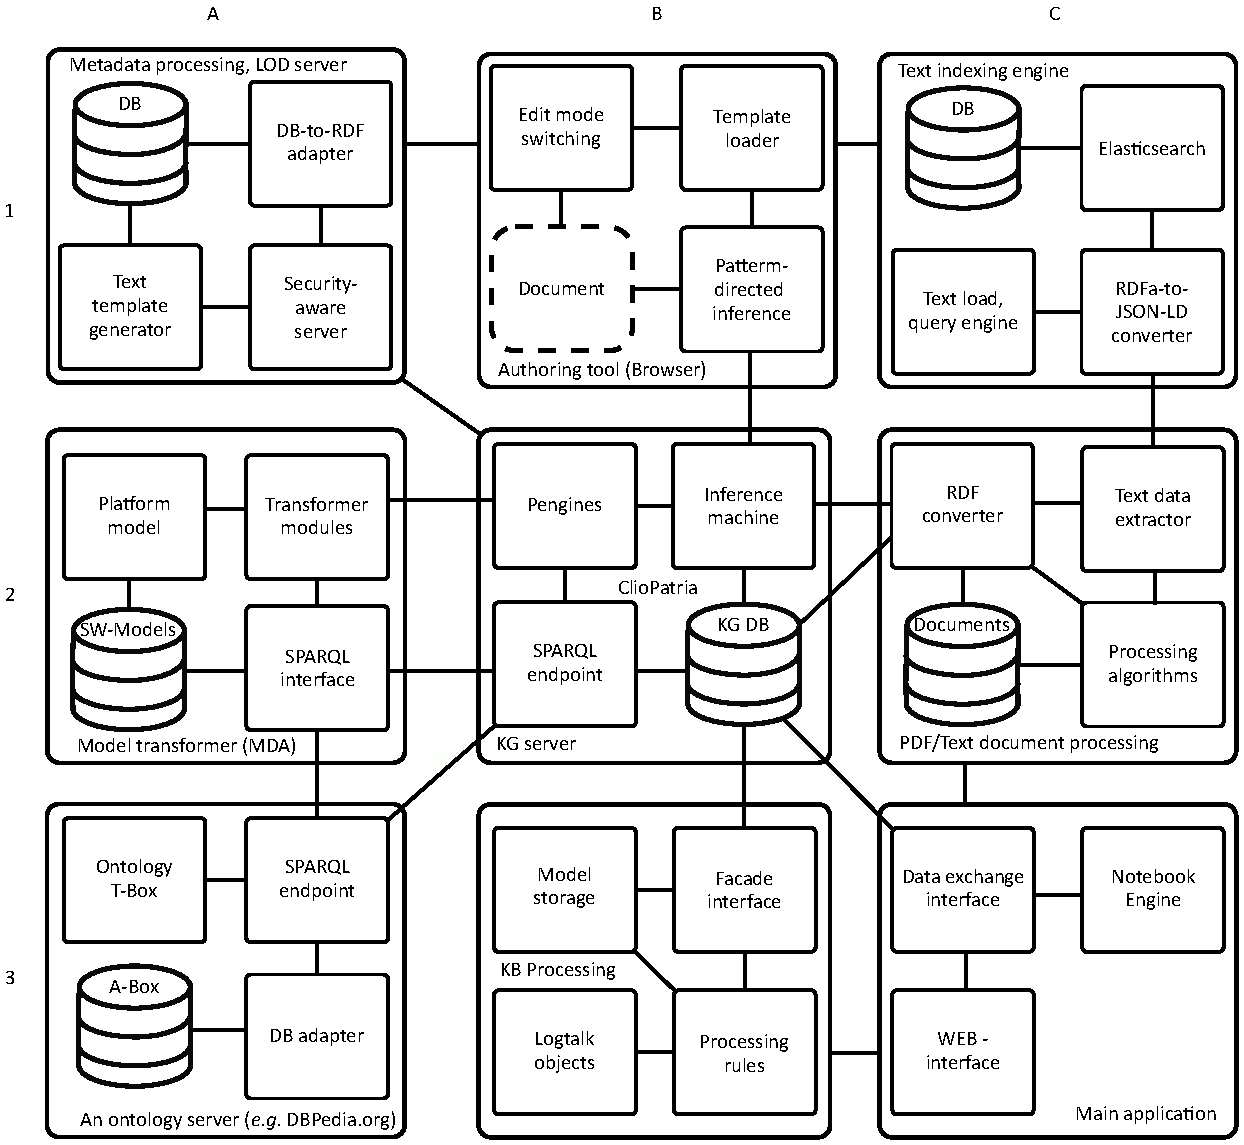
\includegraphics[width=1\linewidth]{architecture-mda-lod-ext-general.pdf}
\caption{Общая архитектура используемой платформы разработки программного обеспечения на базе графа знаний}
\label{fig:arch}
\end{figure}

% Текст надо адаптировать к заджачам.
Ядром приложения строится на доступе к серверу ГЗ (B2), построенному на базе системы Virtuoso, веб-сервере и плагином Pengines~\cite{pengines}. Virtuoso, по сравнению с ClioPatria, поддерживает \verb|UPDATE|- и \verb|DELETE|-запросы языка \verb|SPARQL|, система масштабирума в лоакльной сети. Сервис Pengines позволяет веб-приложениям СВ использовать логический вывод на стороне сервера, интегрировать его со средой JavaScript браузера. База знаний Pengine расширена за счет программных модулей Prolog~\cite{b10,swi}. Граф знаний хранит общую часть A- и T-боксов данных приложений, т.е. это база данных приложений. Другие модули и ресурсы оснащают функции конкретных приложений (C3).

%ClioPatria is a web-application implemented in SWI-Prolog \cite{swi} being ISO-compliant Prolog implementation.  KG functions are implemented with SW package, supplied in standard SWI-Prolog distribution.
Средства создания и интеграции данных документов (B1) -- инструмент, позволяющий реализовать порождение контента документов при помощи технологий СВ, шаблонов и данных с других веб-страниц и веб-сайтов, предоставляющих\footnote{Терминология открытых связанных данных} \cite{b1,c6} ресурсы LOD. Созданная страница храниться в ГЗ в виде набора троек и индексируется в модуле полнотекстовой индексации (C1).

Механизм индексации текста (C1) предоставляет сервис для хранения документов, в JSON, совместно с Virtuoso он позволяет хранить и двоичные объекты в форматах, имеющих текстовый слой. Для модуля существуют две реализации. Одна построена на поисковой системе Sphinx, а вторая — Elasticsearch~\cite{b13}. Elasticsearch использует JSON в качестве единственного формата представления документа.  Данные ГЗ представимы в формате \verb|JSON-LD|, что обеспечивает входные данные для индексирования. Другая реализация основывается Sphinx Search, она намного быстрее индексирует текст и записи базы данных, потребляет меньше оперативной памяти, реализована в языке C++. Выбор движка зависит от основного формата документа, используемого в приложении.

Объекты BLOB, хранящиеся в виде неструктурированных документов ГЗ (PDF-файлы, отсканированные документы), обычно содержат ценные данные, которые должны распознаны и проанализированы для использования в приложении. Такими документами выступают данные отчетов, содержание научных статей, файлы DJVU и растровые изображения. Распознавание данных реализовано в модуле обработки PDF/текстовых документов (C2), здесь производится распознавание и анализ страниц документа, результаты передаются на полнотекстовое идексирование, добавляются в текстовые слои в исходные документы и формируют структуры высокого порядка. Все полученные слои хранятся в базе данных C1, и данные, представляющие особенный интерес, должны быть преобразованы в тройки ГЗ.

Обработка ГЗ общего характера выполняется в модуле B3. Этот компонент задает набор правил, используемых для реализации проверки, вывода эмерджентной семантики, а также анализа и синтеза новых данных, включая выходной результат. Модуль A2 является источником данных об абстрактных моделях (дизайн доменов, UML, постановка задачи и т.п.), которые преобразуются и формируют Т-боксы ГЗ. Преобразование представляет вариант реализации архитектуры, управляемой моделью (MDA, Model Driven Architecture) \cite{b2}. Трансформация осуществляется под управлением модели платформы реализации, задающей контекст преобразования. Например, в случае синтеза исходного кода программного обеспечения модель платформы используется для реализации объектов ООП.

Модуль обработки метаданных (A1) оснащает среду возможностью задания или вывода семантики для выходных данных, порождаемых другими модулями обработки данных. Сервис позволяет сохранять выходные данные в KG для дальнейшего использования в модуле (B3) логического вывода при автоматизации принятия решений. Модуль A3 обозначает собой внешние сервисы и ГЗ с ценными ресурсами, например, обозначениями \cite{b3}глобальных объектов в DBPedia.

\section{Обработка РПД}

Как было сказано выше, входные данные состоят из PDF-документов, представляющих РПД, загружаемых с веб-сайта ИГУ. Сначала документ подвергается анализу, распознаются содержательные данные, которые, затем, могут быть обработаны императивными алгоритмами. Обычно это возможно полноценно реализовать, поскольку PDF-файлы создаются из документов MS Word (не сканируются). Для РПД содержательной информацией является название и код курса, перечень тем, распределение зачетных единиц (академических часов) между лекциями, практикой, семинарами, самостоятельной работой студента, списком вопросов для оценки знаний \emph{и т.д}.

Обработка начинается с преобразования исходного PDF в XML специального формата при помощи библиотеки \verb|Poppler|. Дерево XML обрабатывается объектами, реализованных в виде системы, основанной на знаниях, на \cite{logtalk} объектно-ориентированном (OO) логическом языке программирования Logtalk. Структура исходных данных, представленная в XML-дереве, -- это список страниц с последовательностями кусков текста (run), строк и определений шрифтов. Списки конвертируются в базу данных объекта Logtalk, где каждому элементу задан номер для сохранения исходного порядка, соседние элементы одного типа (шрифт, страница, строка, кусок текста (КТ)) помечены для организации быстрого доступа к рядом стоящим элементам.

Система распознает основные атрибуты (features) каждого КТ (последовательность символов, имеющих общий стиль шрифта) и строки, например, является ли строка висячей строкой абзаца, или присутствует ли число в начале строки. Для всех текстовых строк страницы определяются ограничивающий прямоугольник (bounding box), игнорируя номера страниц (одн- или двусимвольные строки у верхнего или нижнего края страницы с номером, равным номеру страницы PDF). Полученные характеристики используются в объединении КТ и строк в абзацы, ограничивающий прямоуголник также используется для распознавания дополнительных свойств строк. Каждое объединение строк и КТ сопровождается пересчетом геометрических параметров абзаца. Абзацы, разделенные разрывами страниц, реконструируются на втором этапе, используя специальные правила.

Следующим этапом является распознавание структуры разделов РПД. Каждый институт ИГУ поддерживает свои шаблоны для создания РПД, так что последовательности разделов и стили шрифтов заголовков схожи внутри подразделения, но различаются между институтами. Заголовки распознаются по их номерам в исходном шаблоне, сверяясь с последовательностью корней слов, составляющих заголовок раздела. Вариации шаблона учитываются путем указания категории (\verb|category|), задающей специализированные правила и корректирующей параметры общих правил. Затем, все строки/абзацы связываются с предшествующим заголовком. Заголовки и подзаголовки также находятся в иерархических отношениях.  Для каждого заголовка в программе задана его семантика. Итак, на данном этапе документ распознан до деревовидной структуры основных разделов документа и абзацев.

После построения этой иерархии запускается процесс распознавания нумерованных и ненумерованных списков. Здесь предполагается, что маркированные (ненумерованные) списки имеют более глубокий уровень вложенности в сравнении с нумерованными. Процесс состоит из двух этапов: объход всех структур, подобных списку, и поиск общих последовательностей чисел с постоянно увеличивающимися значениями или одинаковых маркировочных символов, пытаясь сохранить возможную вложенность; собственно само свертывание списков. При обнаружении однострочного списка этот случай рассматривается как ложноположительный элемент списка, он присоединяется к предыдущему абзацу в виде обычной строки. Это правило распознает, например, номера страниц в ссылках, оказавшихся при верстке документа на отдельной строке. На этом этапе НИРОКР мы игнорируем списки описаний терминов, начинающиеся с существительного, за которым следует двоеточие или тире.

Последний этап -- это экстракция требуемых данных о РПД. На этом этапе очень важны данные о контекстах, задаваемых семантиками заголовков и структур свертки списков, они ограничивают набор абзацев, в которых расположены нужные данные. Местоположение данных указывается контекстом и списком предшествующих корней слов и знаков препинания. Целевые данные извлекаются с помощью регулярных выражений или других процедур обработки строк.

Основным методами программирования объектов в подсистеме распознавания, используемых при реализации анализа документов, являются расширение и композиция объектов. Исходная XML-структура документа инкапсулируются в виде параметрического объекта Logtalk~\cite{logtalk}, параметром которого является имя временного файла, содержащего XML. Данный бъект предоставляет базовые функции ввода-вывода, преобразование из дерева XML в базу данных объекта, изменение содержимого базы данных с сохранением согласованности, печать сообщений отладки и т.п. Объекты расширяются при помощи импорта набора категорий, реализующих этапы анализа и синтеза, конкретизирующих набор конфигурационных предикатов.  В результате такой композиции создаются объекты, реализующие распознавание структуры кокретного типа документов. Объект распознавания конструируется с учетом свойств конкретного шаблона РПД, система импортированных категорий настраивается под шаблон за счет объектов"=потомков, улучшающих возможности распознавания. По сравнению с существующими компонентными системами программирования в Logtalk конфигурация реализуется теми же программными структурами, что и реализация предикатов, все это благодаря абстрактному синтаксису Prolog/Logtalk.  Более того, параметры конфигурации также могут быть правилами, выводящими значения из существующего контекста. Извлеченные данные сохраняются в локальный ГЗ, который добавляется к удаленному основному ГЗ, хранящему в себе данные учебных планов.

\subsection{Формирование и порождение РПД}

Данные РПД, хранящиеся в ГЗ, помещаются в \LuaLaTeX{} шаблон, реализованный с использованием специального \LaTeX{} класса \verb|sucourse|, подкласс KOMA-скрипта \verb|scrartcl|.  В классе \verb|sucourse| реализованы специальные команды и блоки (environment) для определения распределения учебных единиц между лекциями, практиками и т.п. при помощи ключевых слов. Рассмотрим пример формирования перечня лабораторных работ, выраженных специальными \LaTeX{} блоками.

\begin{minted}{latex}
\begin{labworks}[comp={PC-4,PC-12}] % Компетенции по умолчанию,
                          % удовлетворяемые перечнем лабораторных работ.
. . .                     % Предыдущие лабораторные работы
\begin{work}[comp={PC-4}, % компетенции данной лабороторной работы
    hours=16,             % количество академических часов на работу
    topics={4},           % Набор лекций с материалом для работы
    label=lw:distr]       % Ссылки в терминологии LaTeX \label...
    {Construction of a distributed computational system}
                          % Название лабораторной работы
    \paragraph{Problem definition:}Реализовать среду обработки данных
       типа <<Map-Reduce>> в горизонтальном кластере.
    \paragraph{Дано} результаты предыдущих лабораторных работ.
    \paragraph{Разработать} сеть взаимодействующих сервисов,
       реализующих потоковую (dataflow) архитектуру обработки информации.
    \paragraph{Дополнительное задание} Организовать управление вычислениями
       при помощи сервера RabbitMQ.
\end{work}
\end{labworks}
\end{minted}

Например, лабораторные работы определяются двумя блоками \verb|labworks|, настраивающим блок перечисления лабораторных работ и контекст RDF для сбора данных СВ, \verb|work|, задающим конкретную задачу. Функции блоков определяется так называемым новым \LaTeX{} расширенным синтаксисом \LaTeX2e, позволяющим программисту управлять типами параметров определяемых структурных элементов. Текущая альфа-версия класса \verb|sucourse| опубликована на сайте Github \cite{ghs}.

\begin{minted}{latex}
\NewDocumentEnvironment{works}{O{}} % Определение блока в расширенном синтаксисе
{ % Запускается в точке \begin{...work}
  \def\itemname{Работа студента} % Заготовка газвания работы студента
  \begin{syll@items}[#1]  % Обработка ключевых слов
  \begin{rdfctx}{\rdfsetctx{list}{syll wpdd:itemList % Разметка RDF
       !wpdd:ExampleList !wpdd:CurrentAttestation !wpdd:ItemList}}
  \def\syllabus@worktype{wpdd:LaboratoryWork} % Тип элемента списка в RDF
}
{ % Запускается в точке \end{...work}
  \luadirect{ syll.items:workValidation() } % Запуск проверки табличных данных
\end{rdfctx} % Конец контекста RDF
\end{syll@items} % Конец блока
}

\NewDocumentEnvironment{labworks}{O{}} % Специализация блока ``works''
{
\syl@labwork@section % Начать с адаптера общего шаблона РПД
\begin{works}[totalnames={'hours'},
  type=labwork,      % Разновидность академического часа (лекция, лабораторка
  itemname={Лабораторная работа},  % Задать имя элемента списка
  rdftype={LaboratoryWork},#1]}% Задать тип RDF для элемента
{\end{works}}

\NewDocumentEnvironment{work}{O{}m} % Задать работу с обязательным заголовком
{
  \begin{syll@item}[#1]{#2} % Setup item with a parent assets
  \begin{rdfenv}{list ^schema:member !wpdd:ListItem
     !wpdd:Example \luadirect{self.item:sprintRDFTypes()} }
  \paragraph{{\workheaderstyle \itemname\ \theitem.}~{\worktitlestyle #2}}
     % Формат начала элемента списка
}
{
\end{rdfenv}\par\vspace{1em} % Добавить пустуюстроку между лабораторными
\end{syll@item}
}
\end{minted}


Блоки неявно выполняют \verb|Lua|-код для сбора данных, проверки ограничений и генерации таблиц и других \TeX{} структур РПД. Если логические ограничения не выполняются, в исходный код \TeX{} РПД, транслируемый \LuaLaTeX{}, добавляется сообщение об ошибке в виде текста, окрашенного в красный цвет. Проверку можно отключить при помощи ключевого слова \verb|final| в операторе задания класса \LaTeX"=документа  (ключевое слово \verb|draft| включает отображение результатов проверки целевой PDF, даже если все заполнено правильно). Код Lua также генерирует вспомогательные файлы с данными, обрабатываемими между запусками \verb|lualatex|.

Данная функция используется для проверки наличия печатных изданий в библиотеке университета, обновления и проверки существования URL-ссылок электронных изданий. Эта служба реализована асинхронно при помощи RabbitMQ, организующей рабочие процессы в локальной сети. В одном из подграфов ГЗ хранятся данные изданий и URL-ссылки. Собранные данные из \LaTeX{} УП также отправляются в KG.

Использование \LuaLaTeX{} как основной механизм обработки текста определяется его выдающимися возможностями по качеству верстки документов, высокоуровневой разметкой командами и блоками, доступностью шрифтов True-type и поддержкой Lua, позволяющего расширять функции \LaTeX{} и взаимодействовать с параллельными процессами. Специальные команды не дают пользователю изменять стили, также, определением полезных новых структур можно поддерживать создание документов с общими текстовыми структурами, представляющими различные аспекты учебной программы. Типичным примером являются тесты, интегрируемыми в исходный текст, а затем экспортируемыми в формат, принимаемый системой Moodle.

Начальное состояние \LuaLaTeX{} РПД генерируется программой Python и механизмом шаблонизации Jinja, расширенного функциями поддержки RDF. Jinja расширен синтаксическими структурами, позволяющими запрашивать ГЗ или его локальный подграф для получения данных графа. Расширения реализуют запросы, возвращающие значения некоторого типа (\verb|rdf:type|), блоки обработки набора ответов на запрос и определения нового RDF"=контекста. Результаты предварительной подготовки шаблона также включают семантическую разметку, невидимую в окончательном PDF, но позволяющую экстрагировать данные RDF из исходных текстов \LuaLaTeX{} РПД (аналогично RDFa в HTML).

\section{Планирование расписания}

Проектирование расписания вуза -- известная проблема. В ИГУ сложность решения этой задачи не является большой. Это связано с тем, что многие запросы на расписание трудно формализовать, и они уже рассматриваются при ручном редактировании. В настоящее время расписание составляется нецентрализованно, т.е. отдельно для каждого института или факультета.  Программа формирует расписание только для одного академического подразделения (института).

Чтобы сформировать расписание хорошего качества (максимально удовлетворяющее потребности преподавателей и студенческих групп, минимизирующее ресурсы аудиторного фонда), необходимо учитывать ряд ограничений, таких как запрет на свободные промежутки времени, контроль вместимости аудиторий, различные желания преподавателей, например, в какие дни удобнее проводить занятия, максимальное количество занятий в день и т.д. Не всегда возможно учесть все запросы, поэтому в ИГУ реализована система, генерирующая предварительную версию расписания, позволяющая удобно редактировать результат.

Чтобы рассчитать расписание, ограничения должны быть представлены в структурированном формате, который система способна загружать и обрабатывать. Для формирования набора ограничений, влияющих на расписание, необходимо использовать следующие исходные данные:
\begin{itemize}
\item для класса: количество посадочных мест, наличие проектора, компьютеров \emph{и т.д}.;
\item для преподавателей (предпочтения и запросы):
\begin{itemize}
\item количество рабочих дней в неделю;
\item максимальное количество занятий в день;
\item желаемое расписание занятий в течение учебной недели (компактное, равномерное, без предпочтения);
\end{itemize}
\item для студенческих групп:
\begin{itemize}
\item академическая нагрузка (общее количество академических часов по каждой дисциплине, а также количество занятий в неделю);
\item количество студентов в группах;
\item особенности занятий (потоки, факультативы \emph{и т.д.});
\item фамилия, имя и отчество преподавателя для каждой пары;
\item желаемый класс для конкретного курса.
\end{itemize}
\end{itemize}

% В настоящее время расписание ГИП составляется отдельно каждым подразделением. % Институты ISU составляют расписание с помощью электронных таблиц Excel или делают это полностью вручную на листе бумаги. Программное обеспечение также используется в процессе планирования в других институтах.

% Например, в IMIT ISU для составления расписания используется программа `АВТОМАТИЧЕСКОЕ расписание", которая позволяет пользователю работать с расписаниями различной степени сложности.
% Программа может учитывать ограничения, перечисленные выше.

% Программа `АВТОМАТИЧЕСКОЕ расписание" позволяет максимально облегчить и автоматизировать сложную работу составителей расписания.
% Система помогает легко строить, корректировать и распечатывать расписание в удобном виде и наглядные документы.

% Сложность заключается в том, что такая программа не допускает интеграции с другими университетскими системами, поэтому пользователю приходится вводить все данные об учебном процессе вручную. Все данные учебного процесса хранятся в корпоративной информационной системе ИГУ <1C:University>>. Поэтому наиболее удобным способом интеграции была бы автоматическая загрузка данных об учебном процессе, которые легли бы в основу составления расписания.

% Поскольку программа ''AUTO Schedule'' не имеет открытого API, она не позволяет скачивать данные об учебном процессе, разработка системы планирования с возможностью интеграции с системой <<1C:University>> является актуальной задачей, которую можно было бы выполнить с помощью платформы.

%/GA's /
% A new version of scheduling program must load collected data from ГЗ.

Для достижения этих требований необходимо создать систему, основанную на знаниях, выводящую данные из содержимого ГЗ. Основным источником данных являются УП, планирование нагрузки ППС и описания ресурсов института, имеющие несколько динамический характер (изменяются год от года).

\section{Реализации-аналоги}

В ходе поиска аналогов и работы в сотрудничестве с другими вузами Иркутска и Санкт-Петербурга мы собрали данные об их опыте, которые будут корректироваться под требования ИГУ.

Санкт-Петербургский электротехнический университет (СПбГЭТУ) разработал систему автоматизации разработки учебных программ \cite{leti}. Система позволяет преподавателям вводить значимую информацию о РПД и др. документов в хранилище в формате JSON при помощи заполнения форм. Каждый документ представлен в виде JSON-структуры. РПД генерируются в виде исходного кода \LaTeX{} и преобразуются в PDF. Секретарь кафедры получает PDF-файлы и публикует их на домашней странице курса. Система постоянно развивается в специальном отделе университета. К настоящему времени реализован документооборот и роли сотрудников, в частности, документы проверяются ролью, занимающейся проверкой соответствия стандартам. Состояние обработки документа представлено в пользовательском интерфейсе. Система способна хранить произвольные PDF-документы и генерировать целый пакет документов для представления органам квалификации.

% https://etu.ru/en/university/
Менее совершенныйгенератор разработан в Национальном исследовательском государственном техническом университете (ИрНИТУ) \cite{nrtu} Серверное PHP-приложение содержит учебные планы, сгенерированные программой <<Шахты>>, представляет пользовательский интерфейс для определения формальных частей РПД таких, как темы лекций, список лабораторных работ, самостоятельных работ и семинаров с распределением зачетных единиц между ними. На заключительном этапе генерируется документ Word в формате \verb|docx|.</u0> Данные, не имеющие отношение к УП, должны быть заполнены вручную ежегодно: список тестов, вопросы к экзамену, ссылками на литературу и т.п.

% https://eng.istu.edu/
Аналогичный принцип помощи преподавателям находится в основе подсистемы ИС книгоиздателя «Лан», но их система ориентирована только на автоматизацию сбора электронных изданий для учебной программы РПД. Информационная система хранит все книги, структурированные по множеству тегов предметной области, и предоставляет списки литературы, отфильтрованные по схожим темам, относящимся к набору ранее выбранных экземпляров.

Поиск в Гугл в российской части интернета приводит к большему количеству примеров генераторов учебных планов, их грубый обзор предоставляемых функций в руководствах пользователя выявляет общее направление развития для улучшения возможностей порождение РПД и др. документов. В нашем НИРОКР необходимо создать систему, которая использует существующие структурированные и неструктурированные данные для построения информационной модели образовательного процесса ИМИТ ИГУ, а также масштабирования результатов на другие факультеты.

\section*{Заключение}

На данном этапе исследования нами разработан набор сервисов на базе инфраструктуры с использованием графов знаний и Семантического Веба в качестве центральных технологий интеграции и разработки приложений. Обработка модулей инфраструктуры основана на активном использовании метаданных, распределенных и удаленных семантических ресурсов. Это позволяет построить решение многоагентным способом, где агенты независимы друг от друга, обеспечить общую модель предметной области при проектировании структур данных.

Среди вполне успешных НИРОКР выделены два подпроекта, представленных статье:
\begin{itemize}
\item распознавание структуры данных РПД из PDF-документов и
\item их порождение с использованием данных новой учебной программы.
\end{itemize}
Дальнейшее развитие предполагается вести в двух основных направлениях:
\begin{itemize}
\item повышение качества распознавания РПД за счет автоматизации распознавания таблиц PDF-документов, основанном на открытом ПО наших коллег \cite{Shigarov_2016,Shigarov_2017},
\item внедрение программного обеспечения для составления расписания с использованием данных, полученных на основе собранных данных KG.
\end{itemize}

% TODO: in Conclusion say about RDFa to allow user knowing nothing about LaTeX.

\begin{acknowledgments}
Результаты получены в рамках государственного задания Минобрнауки России, проекта «Методы и технологии облачной сервис-ориентированной цифровой платформы сбора, хранения и обработки больших объемов мультиформатных междисциплинарных данных и знаний на основе использования искусственного интеллекта, модельно-ориентированного подхода и машинного обучения», No.~FWEW-2021-0005. (Государственная регистрация No 121030500071-2).  В проекте использована сетевая инфраструктура Телекоммуникационного центра коллективного пользования «Интегрированная информационно-вычислительная сеть Иркутского научно-образовательного комплекса» (\url{http://net.icc.ru}).</u0>
\end{acknowledgments}


\begin{thebibliography}{99}
\bibitem{zh2020} Z. Stojanov, J. Stojanov, G. Jotanovic, D. Dobrilovic. Weighted networks in socio-technical systems: Concepts and challenges. CEUR-WS Proceedings of the 2nd International Workshop on Information, Computation, and Control Systems for Distributed Environments Irkutsk, Russia, July 6-7, 2020. p.~265--276.
\bibitem{kg} Hogan A., Blomqvist E., Cochez M., D’Amato C. \emph{et al}. Knowledge Graphs -- 2020 URL:\url{https://arxiv.org/abs/2003.02320v5} (access date: 12-Dec-2021)
\bibitem{virtuoso} Erling O. Virtuoso, a Hybrid RDBMS/Graph Column Store // IEEE Data Eng. Bull. 2012. Vol. 35 -- pp.~3--8.
\bibitem{b8}
  J. Wielemaker, W. Beek, M. Hildebrand, J. Ossenbruggen, ClioPatria: A
  SWI-Prolog infrastructure for the Semantic Web, Semantic Web.
  Vol. 7(5). P. 529--541 (2016) \doi{10.3233/SW-150191}
\bibitem{tbl} T.~Berners-Lee, J.~Hendler, O.~Lassila.  The semantic web: A new form of web content that is meaningful to computers will unleash a revolution of new possibilities.  Scientific American, May 2001.
\bibitem{pengines} T.~Lager, J.~Wielemaker. Pengines: Web Logic Programming Made Easy.  Theory and Practice of Logic Programming, volume~14, No.~4-5, 2014, pp.~539--552. \doi{10.1017/S1471068414000192}
\bibitem{b10}
  J. Wielemaker, G. Schreiber, B. Wielinga, Prolog-based infrastructure
  for RDF: scalability and performance, In: D. Fensel, K. Sycara,
  J. Mylopoulos (eds) The Semantic Web -- ISWC 2003. ISWC 2003. Lecture
  Notes in Computer Science. Vol. 2870. Springer, Berlin,
  Heidelberg, 2003.
\bibitem{swi} J.~Wielemaker, T.~Schrijvers, M.~Triska, T.~Lager. SWI-Prolog. Theory and Practice of Logic Programming, volume~12, No.~1-2, pp.~67--96, 2011, ISSN~1471-0684.
\bibitem{authoring} E.~Cherkashin, A.~Shigarov, V.~Paramonov, A.~Mikhailov, Digital archives supporting document content inference, Procs.  of 42-nd International Convention on Information and Communication Technology Electronics and Microelectronics (MIPRO), May 20–24, 2019.  pp. 1037-1042. \doi{10.23919/MIPRO.2019.8757196}
\bibitem{zont19} Cherkashin E., Shigarov A., Paramonov V. Representation of MDA transformation with logical objects // Procs. of International Multi-Conference on Engineering, Computer and Information Sciences (SIBIRCON) Novosibirsk, Russia -- 2019 -- pp.~0913--0918 \doi{10.1109/SIBIRCON48586.2019.8958008}
\bibitem{b1} Ch. Bizer, N. Heath, T. Berners-Lee, Linked data -- the story so
  far, International Journal on Semantic Web and Information Systems.
  2009. Vol. 5 (3). P. 1--22. \doi{10.4018/jswis.2009081901}.
\bibitem{c6} N. Heino, S. Tramp, N. Heino, S. Auer, Managing web content using linked data principles – combining semantic structure with dynamic content syndication, Computer Software and Applications Conference (COMPSAC), 2011 IEEE 35th Annual. pp. 245 - 250.  \url{http://svn.aksw.org/papers/2011/COMPSAC_lod2.eu/public.pdf}
\bibitem{b13}
  R. Kuć, M. Rogoziński, Mastering Elasticsearch - Second edition, Packet
  Publishing. 372 p. (2015)
\bibitem{b2} Cherkashin E., Terehin I., Paramonov V. New transformation approach for Model Driven Architecture // Proceedings of the 35th International Convention MIPRO, Opatija -- 2012 -- pp.~1082-1087.
\bibitem{b3}
  J. Lehmann, R. Isele, M. Jakob, A. Jentzsch, D. Kontokostas, \textit{et al},
  DBpedia -- a large-scale, multilingual knowledge base extracted from
  Wikipedia, Semantic Web Journal. Vol. 6, No. 2, P. 167--195,
  IOS Press (2015)
\bibitem{logtalk}Moura P. Programming Patterns for Logtalk Parametric Objects // In: Abreu, S., Seipel, D. (eds) Applications of Declarative Programming and Knowledge Management. INAP 2009. -- Lecture Notes in Computer Science -- Vol. 6547 -- Springer, Berlin, Heidelberg -- 2011. \doi{10.1007/978-3-642-20589-7_4}
\bibitem{ghs} A \LuaLaTeX{} class for authoring syllabi, URL:\href{https://github.com/eugeneai/sucourse} (access date: 10.10.2022)
\bibitem{leti} ETU “LETI”, URL:\url{https://etu.ru/en/university/} (access date: 10.10.2022)
\bibitem{nrtu} INRTU is a university with the best traditions\ldots, URL:\url{https://eng.istu.edu/} (access date: 10.10.2022)
\bibitem{lanbook} LMS  Lan', URL:\url{} (in Russian) (access date: 10.10.2022)
\bibitem{Shigarov_2016}
A. Shigarov, V. Paramonov, P. Belykh, A. Bondarev, Rule-based canonicalization of arbitrary tables in spreadsheets, In: G. Dregvaite, R. Damasevicius (eds) Information and Software Technologies. ICIST 2016.
\bibitem{Shigarov_2017}
A. Shigarov, A. Mikhailov, ``Rule-based spreadsheet data transformation from arbitrary to relational tables,'' Information Systems, 71, (2017). \doi{10.1016/j.is.2017.08.004}
% \bibitem{GT} Belghiat A., Bourahla M.. UML Class Diagrams to OWL Ontologies: A Graph Transformation based Approach // International Journal of Computer Applications -- Vol. 41 -- pp.~41-46.
\end{thebibliography}

\end{document}

%%
%% End of file

%%% Local Variables:
%%% mode: latex
%%% TeX-master: t
%%% End:
